
There are two major phases in any ``Program Understanding'' tool: \textit{data collection} and \textit{data analysis}.
%
\begin{itemize}
	\item \textit{data collection:} To understand the runtime behavior of applications, an efficient tracing mechanism is required to collect informative data during execution of the application.
	\item \textit{data analysis:} Upon failure or observing unexpected behavior of the program (e.g., a wrong answer), studying the collected execution data would reveal insight about how the program behaved dynamically and what went wrong.
\end{itemize}



In this section, we provide some background that explains our methodology for data collection and data analysis towards debugging and locating potential root causes of the unexpected behavior. 
%

% Binary tracing
\subsection{ParLOT: Efficient Trace Collection}
\label{subsec:parlot}

The executable of HPC applications is often a combination of a large code base and a complex build system with numerous dependencies and libraries.
%
Injecting instrumentation code to the source code is difficult in the HPC space.
%
Also, recompilation of the application with compiler wrappers, as in TAU \cite{tau} and Score-p \cite{scorep}, may break the build system.
%
The instrumentation and tracing mechanism of existing tools are often dependent on other libraries that are need to be present on the target system for trace collection.
%
For example STAT \cite{stat} and AutomaDeD \cite{automaded-laguna} require Dyninst \cite{dyninst} for instrumentation, and MRNet\cite{mrnet} and  TBON\cite{tbon} for providing a distributed communication of tracing mechanism.
%
To enable comprehensive data collection in combination with low time and space overhead, HPC program analysis tools often sacrifice one for the other.
%
However, ParLOT collects whole-program function call traces at as low as library level, while incrementally compressing traces on-the-fly and leaving the majority of the system bandwidth for the application.
%
ParLOT collects \textit{whole} program function call traces with the mindset of \textit{paying a little upfront and saving resource and time cost of reproducing the bug later}.
%
ParLOT instruments the entry and exit point of each function in the binary using Pin \cite{pin} (fig.~\ref{fig.parlotOverview}). 
%
A unique id is assigned to each distinct function at runtime and every time the  function is called (returned), its id is pushed (popped) from the compressed stack.
%
In this fashion, each ParLOT trace contains highly compressed sequence of function calls and returns for every thread of the application code, reflecting the dynamic control flow and call stack.
%
Formally, a ParLOT Trace \textbf{$(PT)$} is a sequence of ordered integers $<f_i,...,f_j>$ where $f_0$ represents a \textit{return} and $f_k$ is the ID of \textit{function k} ($k \neq 0$).
%
Note that $PT_{p.t}$ refers to the $PT$ that belongs to process $p$ and thread $t$ of that process.
%
Enabling ParLOT on top of execution of HPC applications would generate $PT$s for every running thread, enabling analyzers to dig into dynamic behavior of application.
\begin{figure}[t]
\caption{ParLOT Overview}
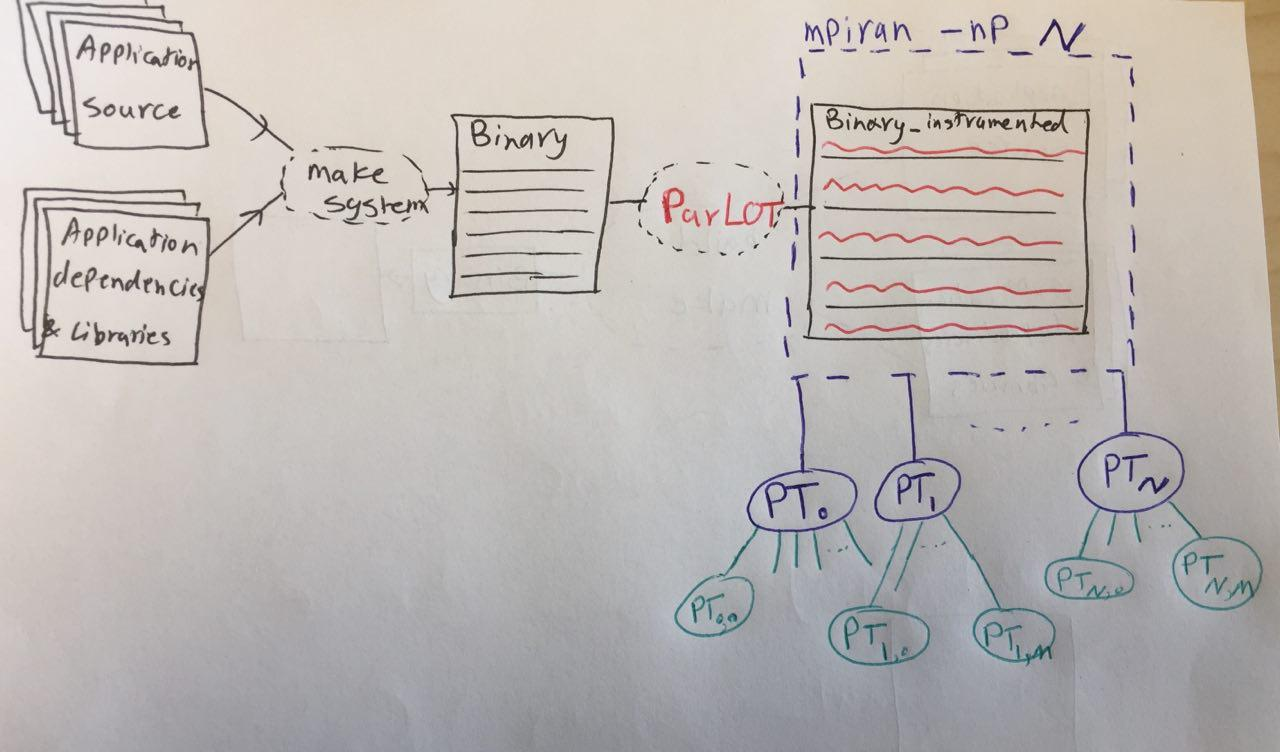
\includegraphics[width=0.45\textwidth]{figs/parlotOverview.jpg}
\label{fig.parlotOverview}
\end{figure}

% NLRs
\subsection{Loop structure detection}
\label{subsec:nlr}

HPC applications and resources are of great interest to scientists and engineers for simulating \textit{iterative} kernels. Computer simulation of fluid dynamics, partial differential equations, the Gauss-Seidel method, and finite element methods in form of stencil codes, all include a main outer loop that iterates over some elements (i.e., timesteps) and updates the elements.
%
This character of typical HPC applications makes PTs very long (often millions or billions of entries) with a relatively small number (hundreds to thousands) of distinct elements (i.e., function IDs).
%
We propose a representation of PT elements (intra-PT compression) in form of \textit{loop structures}, such that PT = sequence of repetitive patterns (i.e., loops). In other words, each PT is a sequence of \textit{Loop Bodies (LB)} that repeated \textit{Loop Count (LC)} times, consecutively.
%

According to Makoto Kobayashi's \cite{kobayashi-84} definition of loops, an occurrence of a \textit{loop} is defined as \textit{a sequence of elements} in which a particular sequence of \textit{distinct elements} (called the \textit{cycle} of the loop) is successively repeated.
%
Later, Alain Ketterlin \cite{Ketterlin-nlr} expanded this definition to numerical values for compressing and predicting memory access addresses and designed the Nested Loop Recognition (NLR) algorithm.
%
The basic idea behind the NLR algorithm is that a linear function model can be extracted from the linear progression in a sequence of numbers, and these linear functions form a tree in which the depth of each node is the depth of a \textit{nested} loop (the outermost loop's function is the root of the tree with depth 0).
%
We have modified the NLR algorithm to make it suitable for PTs.
%
Each repetitive pattern and its frequency of consecutive appearances would be compressed to a single \textit{Loop Structure (LS)} entry.
%
\begin{definition}{Loop Structure} $LS = LB \; \hat{} \; LC$ where $LB  = <pt_i,...,pt_j>$ ($0 <= i < j < len(PT)$) that occur $LC$ times is in a sub-sequence $<pt_i,...,pt_k>$ ($k = 3j, k < len(PT)$)

\end{definition}
%
By converting each PT into a sequence of $LS_i$, we reduce the length of PT by a factor of $\sum_i len(LB_i) * LC_i$. 
%

\begin{figure}[]
\caption{Sample NLR}
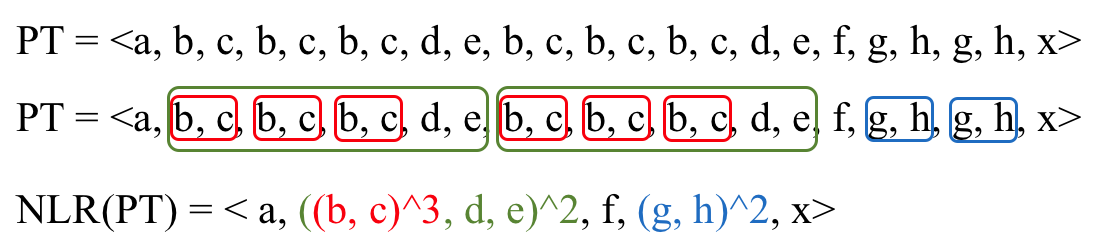
\includegraphics[width=0.45\textwidth]{figs/NLRexample.png}
\label{fig.NLRexample}
\end{figure}

As an example, figure \ref{fig.NLRexample} shows how the sample PT with length 23 can be reduced to 5 after detecting its loop structures.
%
In addition to reducing the size of easy-to-read PTs, NLR can also help with detecting broken loop structures due to a bug. 
%
For example, when a node fails to send or receive messages in a supercomputer after some number of iterations, the PTs that belong to that node would show loop structures with loop counts lower than what was expected. 
%
In other word, NLR is enabling us to ``measure progress'' of each PT and detecting the cause of divergence in the control flow that leads to failure.
%
Later we will explain how this lossless representation of PTs eases the process of diffing between a pair of PTs.

% CLs
\subsection{Equivalencing behavior via FCA}
\label{subsec:fca}
Thanks to ParLoT compression mechanism, we are able to efficiently (w.r.t. time and space) collect whole-program function call and return traces (PTs). However, post-mortem analysis of the PTs from thousands of threads requires decompression of traces, and consequently, analysis of large amount of data. Before jumping into \textit{the huge haystack} of PTs to find \textit{the tiny needle} (bug, bug manifestation or root cause of the failure), a middle ground data manipulation is required to simplify and organize the haystack. 

Reducing the search space from thousands of PTs to just a few groups of equivalent PTs (i.e., inter-PT compression) not only requires a similarity measure based on a call matrix but also a scheme that is efficient even for large process counts.
%
Since a pair-wise comparison of all processes is highly inefficient, we use \textit{concept lattices} that stem from \textit{formal concept analysis} (FCA) \cite{clbook} to store and compute groups of similar PTs.
%
FCA can efficiently split the large haystack into a few hay(semi)stacks with ``conceptually'' similar hays in each. This way conceptually isolated PTs (i.e., outliers) which are the potential bug manifestation or root cause would be detected. If no outlier detected, we only have a few distinct group of PTs to dig in, instead of thousands of large traces. With a wider perspective, here are other benefits of FCA for HPC debugging:
\begin{itemize}
\item FCA is scalable and efficient. It can be built incrementally and different kind of information such as full Jaccard Similarity Matrix (JSM) can be generated in linear time due to CL properties.
\item Clustering is only one advantage of creating concept lattices from ParLoT traces. CLs can integrate all traces from an execution to a single entity as signature/model of good or bad execution for further analysis (e.g., prediction) 
\item Due to the \textit{partial order} of nodes within CLs, valuable information can be retrieved from CLs like Happens-Before relation (Vijay Garg’s book explains all applications of FCA in computer science applications)\cite{latticeForDistConst} and machine learning and data mining \cite{Ignatov17})
\end{itemize}

A concept lattice is based on a \textit{formal context} \cite{clbook}, which is a triple $(O, A, I)$, where $O$ is a set of \textbf{objects}, $A$ a set of \textbf{attributes}, and $I \subseteq O \times A$ an incidence relation. The incidence relation associates each object with a set of attributes (e.g., table \ref{tab:sampleContext}).
%
Using FCA for clustering giving us the capability of clustering trace objects based on the ``concept'' of each trace object. We can characterize the ``concept'' (i.e., what we want to understand from the collected traces) by extracting meaningful ``attributes'' from traces. 
%
However, since we are only interested in grouping similar PTs in this work, we only take advantage of similarity measures \cite{Alqadah2011} of concept lattices and leave other properties for future work.
%
Due to typical HPC application topologies such as SPMD, master/worker and odd/even where multiple processes/threads behave similarly, our experiments show that large numbers of PTs can be reduced to just a few groups.
%

\subsubsection{Concept Lattice Construction}
\begin{itemize}
\item Batch vs. Incremental \cite{clconst}
\item Complexity: $O(2^{2K}||E||)$ where $K$ is an upper bound for number of attributes (e.g., distinct function calls in the whole execution) and $||E||$ is the number of objects (e.g., number of PTs).
\end{itemize}

\subsubsection{FCA example}

Executing the sample code below would result in PTs with the context in table \ref{tab:sampleContext}.

\begin{frame}{}
  \lstset{language=C}
 \begin{lstlisting}
main(){
 int rank;
 int src;
 MPI_Init()
 MPI_Comm_size(MPI_COMM_WORLD)
 MPI_Comm_rank(MPI_COMM_WORLD,&rank)
 if (rank != 0) {
  MPI_Send(0) // Send to rank 0
 } else{ /* rank = 0
  MPI_Recv(1) // Receive from rank 1
  MPI_Recv(2) // Receive from rank 2
  MPI_Recv(3) // Receive from rank 3
 }
 MPI_Finalize()
}
\end{lstlisting}
\end{frame}



\begin{table}[]
\label{tab:sampleContext}
\caption{Context}
\scalebox{0.6}{
\begin{tabular}{l|cccccc}
 & \multicolumn{1}{l}{MPI\_Init()} & \multicolumn{1}{l}{MPI\_Comm\_Size()} & \multicolumn{1}{l}{MPI\_Comm\_Rank()} & \multicolumn{1}{l}{MPI\_Send()} & \multicolumn{1}{l}{MPI\_Recv()} & \multicolumn{1}{l}{MPI\_Finalize()} \\ \hline
Rank 0 & $\times$ & $\times$ & $\times$ &  & $\times$ & $\times$ \\
Rank 1 & $\times$ & $\times$ & $\times$ & $\times$ &  & $\times$ \\
Rank 2 & $\times$ & $\times$ & $\times$ & $\times$ &  & $\times$ \\
Rank 3 & $\times$ & $\times$ & $\times$ & $\times$ &  & $\times$
\end{tabular}}
\end{table}


\begin{figure}[t]
\centering
\scalebox{0.5}{
\includegraphics[width=3.4in]{figs/{sample}.pdf}}
\caption{Sample Concept Lattice from Obj-Atr Context in table\ref{tab:sampleContext}}
\label{fig:sampleCL}
\end{figure}

\begin{figure}[t]
\centering
\scalebox{0.5}{
\includegraphics[width=3.4in]{figs/{sample-reduced}.pdf}}
\caption{Concept Lattice with reduced labels}
\label{fig:sampleCL}
\end{figure}





\subsubsection{Jaccard Similarity Scores}

\begin{itemize}
\item Some background about Jaccard Similarity Score
\item How to obtain full pair-wise Jaccard Similarity Matrix (JSM) from a concept lattice (e.g., LCA approach)
\end{itemize}

\begin{figure}[]
\centering
\scalebox{0.8}{
\includegraphics[width=3.4in]{figs/{fancy1}.pdf}}
\caption{Pair-wise Jaccard Similarity Matrix (JSM) of MPI processes in Sample code}
\label{fig:jsm}
\end{figure}


%\subsection{Ranking Suspicious PTs}
%\label{subsec:ranking}
%\begin{itemize}
%\item Filters
%\item Attributes
%\item 
%\end{itemize}

\subsection{diffNLR: Reflecting differences}
\label{subsec:diffnlr}
\begin{itemize}
\item Inspired by \texttt{diff} original algorithm\cite{diff-myers} that has bin used in Git and GNU Diff, we visualize the differences of a pair of PT as shown in fig \ref{fig:sampleDiffNLR}.
\item This visualization reflects of the differences of \textbf{occurrences} of PT elements and their \textbf{orders}.
\item In section \ref{sec:experimental} we show how this visualization can help us locating the points of divergence in PTs, and potential bug manifestation and root cause.
\end{itemize}

\begin{figure}[]
\centering
\scalebox{0.5}{
\includegraphics[width=3.4in]{figs/{sampleDiffNLR}.png}}
\caption{Sample diffNLR}
\label{fig:sampleDiffNLR}
\end{figure}


